\chapter{Il progetto di tesi: SchoolGPT}
In questo capitolo si andrà a presentare il progetto di tesi, ovvero SchoolGPT, una proof of concept di un sistema di information retrieval per documenti relativi all'ambito didattico.
Tale PoC si prefigge l'obiettivo di dimostrare come i più recenti sviluppi delle tecnologie in ambito NLP possano essere utilizzati da studiosi e ricercatori per ottenere una interfaccia molto naturale e semplice per la ricerca di informazioni, e dei documenti che le contengono, e da aziende per avere dei veri e propri ``consulenti'' virutali a cui chiedere sia informazioni di business o burocratiche che consigli in ambiti tecnici. 

Il progetto è stato sviluppato in Python su notebook Jupyter ed eseguito su Google Colab, per ragioni di costi e hardware necessario. 
La libreria principale è stata LangChain per la creazione di una catena di Question Answering, inoltre sono stati sfruttati dei tool messi a disposizione dalla libreria per realizzare anche l'ingestion del dataset.
\section{L'idea}
Un sistema di information retrieval (IR) è progettato per recuperare informazioni rilevanti da un vasto insieme di dati in risposta a una specifica query posta dall'utente. 
Dal 30 novembre 2022, OpenAI con il suo ChatGPT ha rivoluzionato la concenzione che c'era nell'opinione pubblica riguardo l'intelligenza artificiale e il suo potenziale. Anche a livello accademico c'è stato un grande interesse sui risultati ottenuti da OpenAI, e questo ha portato a un'accelerazione della ricerca e dello sviluppo di Large Language Models (LLM).
Questi modelli sono in grado di generare testi coerenti e pertinenti, e sono in grado di rispondere a domande poste in linguaggio naturale. 
Queste caratteristiche potrebbero essere utilizzate per migliorare i sistemi di information retrieval, consentendo agli utenti di interagire con i motori di ricerca in modo più naturale e ottenere risultati più pertinenti.
Qui di seguito, si elencano i vantaggi dell'usare un LLM in questo contesto:
\begin{itemize}
    \item Ricerca basata sulla comprensione del linguaggio: 
    A differenza dei tradizionali motori di ricerca che fanno corrispondenze di parole chiave,
     un LLM può comprendere meglio il significato implicito e il contesto delle richieste degli utenti.
      Può analizzare e interpretare in modo più accurato le domande poste in linguaggio naturale, 
      contribuendo a fornire risultati di ricerca più pertinenti.
    \item Query estese e complesse: GPT-3.5 e simili LLM possono elaborare query complesse e fornire risposte estese. Ciò significa che un sistema di information retrieval basato su LLM potrebbe non solo restituire link a pagine web, ma anche presentare risposte complete alle domande dell'utente, consentendo una comprensione più approfondita del contenuto.
    \item 
    Personalizzazione dell'esperienza di ricerca: Un LLM può apprendere le preferenze e le esigenze dell'utente nel tempo, adattando i risultati delle ricerche in base ai suoi interessi e comportamenti passati. Ciò potrebbe migliorare l'esperienza dell'utente e rendere i risultati di ricerca più pertinenti.
    \item Ricerca semantica: Grazie alla sua capacità di comprendere il significato del testo, un LLM può identificare correlazioni e relazioni semantiche tra diverse fonti di informazione. Questo potrebbe portare a una migliore scoperta di contenuti pertinenti che potrebbero essere stati trascurati da sistemi di ricerca tradizionali.
    \item 
    Generazione di estratti e riassunti: Un LLM potrebbe estrarre automaticamente le parti più rilevanti e informative di un documento o una fonte e presentarle come riassunto. Questo aiuterebbe gli utenti a ottenere una panoramica veloce delle informazioni senza dover leggere l'intero contenuto.

    \item Ricerca multilingue e comprensione interlinguistica: Un LLM addestrato in più lingue potrebbe consentire una ricerca efficace in diverse lingue, agevolando la scoperta di contenuti in tutto il mondo.

    \item 
    Affinamento dei risultati: Un LLM potrebbe interagire con l'utente per affinare i risultati di ricerca attraverso domande di follow-up, assicurandosi di comprendere meglio le sue intenzioni e fornendo risultati più mirati.
    
\end{itemize}
\section{Il dataset}
Il dataset contiene 33 manuali e libri di testo scolastici, con una media di 226 pagine, pubblicati tra il 1843 e il 1918 in Canada, Stati Uniti d'America e Gran Bretagna.

La maggior parte dei libri parlano di storia e geografia con alcune eccezioni che parlano di ortografia e grammatica tedesca e inglese.

Essendo libri molto datati, la lingua utilizzata, l'inglese, non è quella attuale, ma una versione più antica e formale.

Questa formalità si riscontra anche nella forma che viene utilizzata, in alcuni libri le lettere iniziali dei paragrafi sono molto grandi e decorate, in altri sono in grassetto, in altri ancora sono in corsivo.

Le caratteristiche riportate sopra rendono complicata la creazione di un sistema di Information Retrieval classico che 
sia in grado di restituire risultati pertinenti anche perché le query espresse non sono strettamente nel linguaggio utilizzato nei libri.
Grazie alle capacità linguistiche e di correzione degli errori ortografici dei modelli di LLM è possibile superare questi problemi senza preoccuparsi troppo di ingegnerizzare il dataset da un punto di vista linguistico.

\section{Langchain}
LangChain è un framework per lo sviluppo di applicazioni basate su modelli linguistici.

Il framework non si limita ad offrire un'interfaccia per l'uso di modelli linguistici, ma offre anche un'interfaccia per realizzare applicazioni:

\begin{itemize}
    \item Che sappiano utilizzare informazioni che non sono state oggetto del training, tramite database esterni o internet
    \item Che sappiano interagire con gli strumenti che uno sviluppatore gli mette a disposizione
\end{itemize}

Il framework LangChain offre due principali strumenti:

\begin{itemize}
    \item Componenti: LangChain fornisce astrazioni modulari per i componenti necessari a lavorare con i modelli linguistici. LangChain ha anche collezioni di implementazioni per tutte queste astrazioni. I componenti sono progettati per essere facili da usare, indipendentemente dall'utilizzo del resto del framework.
    \item Catene specifiche per i casi d'uso: Le catene possono essere pensate come l'assemblaggio di questi componenti in modi particolari, al fine di realizzare al meglio un particolare caso d'uso. Sono intese come un'interfaccia ad alto livello attraverso la quale si può facilmente iniziare a lavorare con un caso d'uso specifico. Queste catene sono anche progettate per essere personalizzabili.
\end{itemize}

\subsection[I componenti]{I componenti}
I componenti sono i mattoni fondamentali di LangChain.
Sono progettati per essere facili da usare e integrare, indipendentemente dall'utilizzo del resto del framework.
La prima tipologia di componenti che offre LangChain sono gli \textbf{schema}.
\subsubsection*{Schema} Gli schema sono il modo in cui LangChain rappresenta il testo e le interazioni che si possono avere con i modelli.

Negli schema ci sono quattro tipologie di oggetti:
\begin{itemize}
    \item \textbf{Prompts}: I prompts possono essere semplici stringhe o oggetti più complessi. Tra i prompts più utilizzati i \textit{PromptsTemplate} \label{PromptsTemplate}, ossia delle stringhe che possono essere completate da valori dinamici tramite dei placeholder e i \textit{ChatPromtsTemplate} che sono delle chat sotto forma di template. 
    \item \textbf{ChatMassages}: Sono tipologie di messaggi che rappresentano, letteralmente, una chat con un language model. Possono essere composti da 3 tipologie di messaggi: \textit{SystemChatMessage}, messaggi che rappresentano delle informazioni di contesto per il modello; \textit{HumanChatMessage}, i messaggi che un utente ha inviato al modello; \textit{AIChatMessage}, le risposte che il modello ha inviato all'utente.
    \item \textbf{Examples}: Sono esempi di input e output che possono essere utilizzati sia per il training di un modello, come esempi da imparare, che per la valutazione sia del modello che di una chain dopo aver ottenuto il risultato.
    \item \textbf{Documents}: Rappresentano dei documenti che il modello può utilizzare. Possono essere utilizzati per dividere documenti reali in parti, inserirle in un database e poi essere interrogati.
\end{itemize}

Questi Schema sono i mattoni fondamentali con cui si vanno poi ad utilizzare il secondo tipo di componenti: i \textbf{modelli}.

\subsubsection*{Modelli}
I modelli sono gli oggetti con cui il framework LangChain rappresenta i modelli linguistici e le API con cui interagire con essi.

Il framework divide i modelli in due categorie:
\begin{itemize}
    \item \textbf{Modelli di linguaggio}: Sono modelli che hanno come scopo quello di generare testo. Possono essere utilizzati per generare testo a partire da un prompt, per completare un prompt o per generare testo a partire da un documento.
    \item \textbf{Modelli di chat}: Sono modelli che hanno come scopo quello di simulare una conversazione. 
\end{itemize}

I modelli supportati dal framweork possono essere sia derivanti da soluzioni commerciali come quelli di OpenAI, sia modelli sviluppati dalla community opensource se messi su HuggingFace.
Nell'implementazione in python, tutti i modelli vengono utilizzati come funzioni che ricevono in input una stringa.
Per una lista completa delle integrazioni già supportate si può visitare il link \url{https://python.langchain.com/docs/integrations/llms/}.

\subsubsection*{Indici}

Gli indici si riferiscono alle modalità per strutturare i documenti in modo che i modelli di linguaggio di grandi dimensioni possano interagire al meglio con essi.

Per indici si intendono memorie esterne che il language model può interrogare.

Il modulo riguardante gli indici include anche una serie di strumenti per maneggiare i documenti, tra i quali:

\begin{itemize}
    \item \textbf{Document loaders}: Sono classi e funzioni che caricano i documenti da una sorgente esterna, possono essere pdf, file di testo, pagine web oppure personalizzati. La lista completa si trova al link \url{https://python.langchain.com/docs/integrations/document_loaders/}
    \item \textbf{Text splitters}: Sono classi e funzioni che prendono in input un testo (o documento) molto lungo e lo dividono in parti più piccole. La divisione può esser fatta in molti modi, dal banale carattere alla più complessa divisione in frase o paragrafi semanticamente significativi. La divisione in chunk più piccoli è necessaria per prendere i vettori degli embeddings più precisi e quindi facilitare il lavoro dei retriever.
    \item \textbf{Retrievers}: Sono classi che prendono in input un testo e restituiscono un sottoinsieme di documenti che sono rilevanti per il testo in input. I retriever possono essere utilizzati per trovare i documenti che contengono le informazioni necessarie per rispondere a una domanda.
    \item \textbf{Vector stores}: Sono le classi che permettono l'interazione con un database di vettori e la relativa modalità di interrogazione, possono essere utilizzati direttamente oppure tramite un retriever. Ogni database di vettori mette a disposizione una classe che ha firme comuni alle altre e può essere utilizzato in LangChain.
\end{itemize}

Un altro tipo di memorie invece sono ciò che LangChain chiama ``Memory''.

\subsubsection{Memory}
Quando si parla di ``Memory'' in LangChain ci si riferisce alla memoria, o meglio uno stato, della conversazione fin'ora che c'è stata tra l'utente e un modello.

Questo tipo di memoria viene appesa ad ogni input dato all'utente, eventualmente aggiornata, ed è quindi utilizzata per lo più per contenere informazioni di contesto.

I dati che vengono presi da un vector database sono inseriti in questo tipo di memoria per poi esser letti dal modello e utilizzati per generare una risposta.

Essendo una memoria inserita nell'input, consuma token.

Tutti questi elementi sono la base su cui si basano i due componenti più importanti di LangChain: le \textbf{catene} e gli \textbf{agenti}.

\subsubsection*{Catene}

Per ``catena'' si intende un'interfaccia ad alto livello che permette di utilizzare una serie di componenti, modelli (diversi e non) o addirittura altre catene in modo più o meno sequenziale.

Le catene più comuni sono quelle denominate LLMChain, che combinano un \hyperref[PromptsTemplate]{PromptsTemplate} seguito da un modello e eventualmente un parser dell'output per trasformarlo in un formato diverso.

Altra tipologia molto importante di catena, che è anche la tipologia di catena utilizzata per realizzare il lavoro di tesi, è quella che ha a corredo l'interazione con un retriever e quindi con un index.
Questa tipologia di catene, al momento, ha quattro configurazioni principali che si riferiscono a come la catena interagisce con i documenti ricevuti da un retriever:
\begin{itemize}
    \item \textbf{Stuff}: è la tipologia più semplice, in cui si prendono i documenti correlati con l'input dell'utente e li si inserisce nella memoria della conversazione. Ha come principale pro la semplicità dell'utilizzo e il costo, dato che viene fatta una sola chiamata al modello.
    Come contro principale ha il fatto che tutti i LLM hanno una lunghezza massima di input e se i documenti (o chunk di documenti) sono troppo lunghi si potrebbero avere problemi di infattibilità della richiesta. 
    \item \textbf{Map reduce}: proprio come l'algoritmo utilizzato nel mondo hadoop per il calcolo distribuito, questa tipologia di catena esegue la query su ogni documento ricevuto dal retriever e poi aggrega le varie risposte in un unico testo che viene restituita come risposta.
    Questo tipo di catene non ha problemi di scaling, dato che ogni richiesta viene fatta su un singolo documento, ma risulta anche il suo contro principale dato il costo più alto, inoltre è possibile che si perdano informazioni realizzando l'aggregazione.
    \item \textbf{Refine}: l'algoritmo utilizzato è proprio quello di refine, ovvero si prende il primo documento, si fornisce una prima risposta alla query dell'utente e poi ogni documento successivo aggiorna la risposta migliorandola con nuove informazioni derivanti dal nuovo documento.
    Questo tipo di catene ha come pro il fatto che non si perdono informazioni e che il costo è più basso rispetto a map reduce, ma ha come contro il fatto che non è possibile parallelizzare in modo semplice, dato che la risposta deve essere aggiornata sequenzialmente.
    \item \textbf{Map-Rerank}: diversamente dagli altri algoritmi questa tipologia di catene non combina più documenti per dare una singola risposta ma esegue la query su tutti i documenti e fa una classifica della risposta che, secondo il LLM, è più completa. La migliore viene poi restituita come risposta.
    Come costi è simile al refine, ma ha dei casi d'uso diversi dai precedenti, infatti questa tipologia è utilizzabile quando si sa che la risposta migliore è sempre contenuta in un unico documento. 
\end{itemize}

Per la realizzazione della tesi è stata utilizzata la tipologia di catena ``Refine'' poiché i libri trattano per lo più argomenti simili e quindi è possibile che la risposta migliore esca fuori dal miglioramento della prima risposta che si trova.

\subsubsection*{Agenti}

Alcune applicazioni hanno casi d'uso che non possono essere realizzati con una singola catena, ma hanno bisogno di un sistema più complesso e meno lineare.

Per questi casi nascono gli agenti, ovvero una serie di modalità di interrogare un LLM in modo tale che sia lui a decidere i prossimi passi da realizzare all'interno di un ragionamento più ampio.

Langchain offre gli strumenti necessari per implementare gli agenti, nel dettaglio:

\begin{itemize}
    \item \textbf{Agent}: è l'interfaccia che rappresenta un agente, è un wrapper attorno ad un modello che prende in input un testo e restituisce la prossima azione da svolgere.
    \item \textbf{Tool}: sono funzioni che rappresentano delle azioni che un agente può effettuare, questo tipo di azioni possono essere funzioni python anche molto complesse e includere, per esempio, anche chiamate ad altri llm o agenti. Sono il modo in cui un programmatore può iniettare codice all'interno del ragionamento di un modello.
    \item \textbf{Tollkits}: sono aggregazioni di tool. Sono necessari quando i tool sono molti e, dato il limite di token in ingresso dei modelli, si vuole rendere più leggero il contesto.
    \item \textbf{Agent Executor}: sono le classi che mettono insieme i tool e gli agenti, sono loro che realizzano il ragionamento e coordinano le azioni del agent.
\end{itemize}

Gli agenti possono essere di vario tipo che possono performare meglio su alcune tipologie di task rispetto ad altre, per una lista completa si può visitare il link \url{https://python.langchain.com/docs/modules/agents/agent_types/}.

Nel lavoro di tesi non è stato utilizzato un agente ma, sicuramente, in sviluppi futuri si potrebbe pensare di utilizzarne uno per migliorare l'esperienza utente.

\subsection[Chain specifiche]{Le chain ad uso specifico}
\section{L'implementazione}
L'intero lavoro di tesi è stato svolto in Python\cite{python}, utilizzando un notebook Jupyter\cite{jupyter} come ambiente di esecuzione.

Le librerie selezionate per il progetto sono state di fondamentale importanza per il raggiungimento degli obiettivi prefissati:
\begin{itemize}
    \item \textbf{pypdf}: Questa libreria è stata impiegata per l'estrazione accurata del testo da documenti in formato PDF, consentendo così di lavorare con il contenuto testuale essenziale.
    \item \textbf{pandas}: Essenziale per la gestione efficiente del file XLSX contenente i metadati dei documenti. La flessibilità di Pandas ha facilitato la manipolazione e l'analisi dei dati correlati.
    \item \textbf{tiktoken}: L'implementazione del byte pair encoding (BPE) e della tokenizzazione tramite Tiktoken è stata cruciale per la preparazione dei testi e la loro successiva elaborazione nei modelli di OpenAI. 
    \item \textbf{openai}: La libreria ufficiale di OpenAI è stata utilizzata per interagire con i modelli e le API di OpenAI, consentendo un'interazione agevole e l'integrazione dei risultati nei processi di analisi.
    \item \textbf{langchain}: Questa libreria, che può essere considerata a tutti gli effetti un framework, è stata il fulcro centrale del lavoro di tesi. Grazie ad essa è stato possibile arricchire le capacità di un large language model con concetti avanzati, i quali saranno dettagliatamente esposti in seguito.
    \item \textbf{chromadb}: L'utilizzo della libreria ufficiale di ChromaDB ha consentito la conservazione e l'efficace interrogazione dei vettori di embeddings, rappresentando un passo cruciale per l'analisi e l'elaborazione dei dati ottenuti.
\end{itemize}

Il notebook è stato eseguito su piattaforma Google Colab, che oltre all'esecuzione permette di accedere allo storage di google drive, dove è stato conservato il dataset, in modo semplice e veloce come se fosse una directory della macchina in cui gira il notebook.

L'attenta scelta e l'integrazione di queste librerie hanno fornito gli strumenti necessari per l'elaborazione accurata e la valorizzazione dei dati, contribuendo significativamente al raggiungimento degli obiettivi di ricerca.

L'implementazione del progetto è stata suddivisa in due fasi principali: ingestion e inferenza.

\subsection{Ingestion} 
La fase di ingestion dei dati è descritta dal diagramma di flusso in figura 4.1:
\begin{figure}[H]
    \centering
    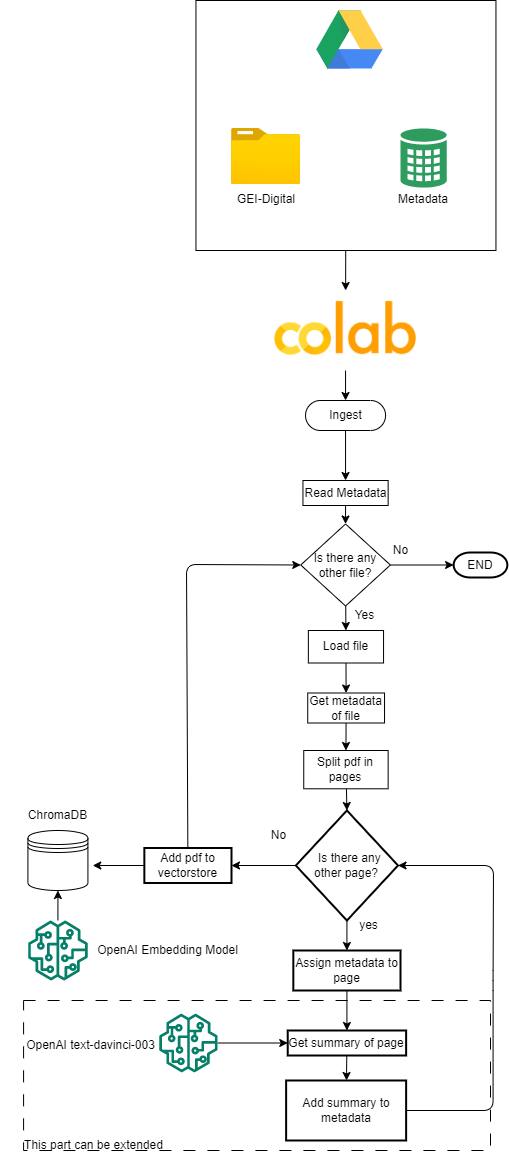
\includegraphics[height=0.5\pdfpageheight]{images/ingest.png}\label{fig:ingest}
    \caption[Ingestion]{Il diagramma di flusso che descrive la fase di ingest dei dati.}
\end{figure}

Come si può osservare, i dati sono stati conservati su Google Drive e il job di ingestion si occupa di leggere i 33 libri in formato pdf,
suddividerli in pagine assegnando loro le informazioni derivanti dai metadati, è presente inoltre una parte di enrichment di tali informazioni 
utilizzando il Large Language Model ``text-davinci-003'' di OpenAI per estrarre un riassunto di ogni pagina. Quest'ultima parte di enrichment è possibile espanderla ulteriormente
utilizzando l'LLM per estrarre ulteriori informazioni, come ad esempio le entità presenti in ogni pagina, ma per il momento è stata tralasciata.
La fase di enrichment inoltre serve ad arricchire i metadati di informazioni che, in seguito, il self-query retriever potrà utilizzare per interrogare il database.

Alimentato il database con le informazioni estratte, è possibile passare alla fase di inferenza.

\subsection[Inferenza]{Inferenza e interazione con l'utente}

La fase di inferenza e interazione con l'utente è descritta dal diagramma di flusso in figura 4.2:

\begin{figure}[H]
    \centering
    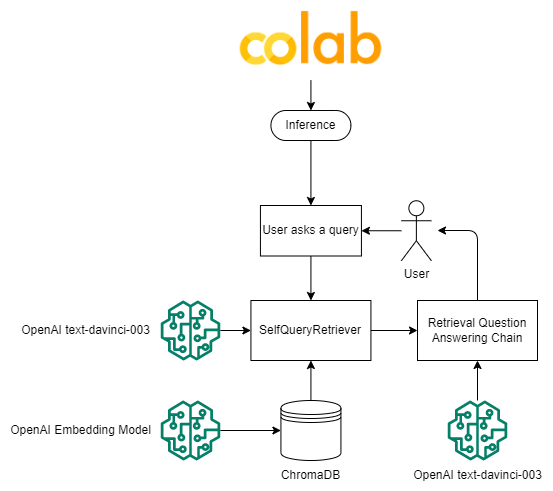
\includegraphics[height=0.3\pdfpageheight]{images/Inference.png}\label{fig:infer}
    \caption[Ingestion]{Il diagramma di flusso che descrive l'interazione dell'utente con il sistema di question answering.}
\end{figure}

Il job di inferenza si occupa di ricevere dall'utente una query in linguaggio naturale, la query passa in input al SelfQueryRetriever, 
che si occupa di interrogare il database e tramite una combinazione di selfquerying (riferimento ~\ref{fig:selfquery}) e similarity research restituisce una lista di documenti.
\begin{figure}
    \centering
    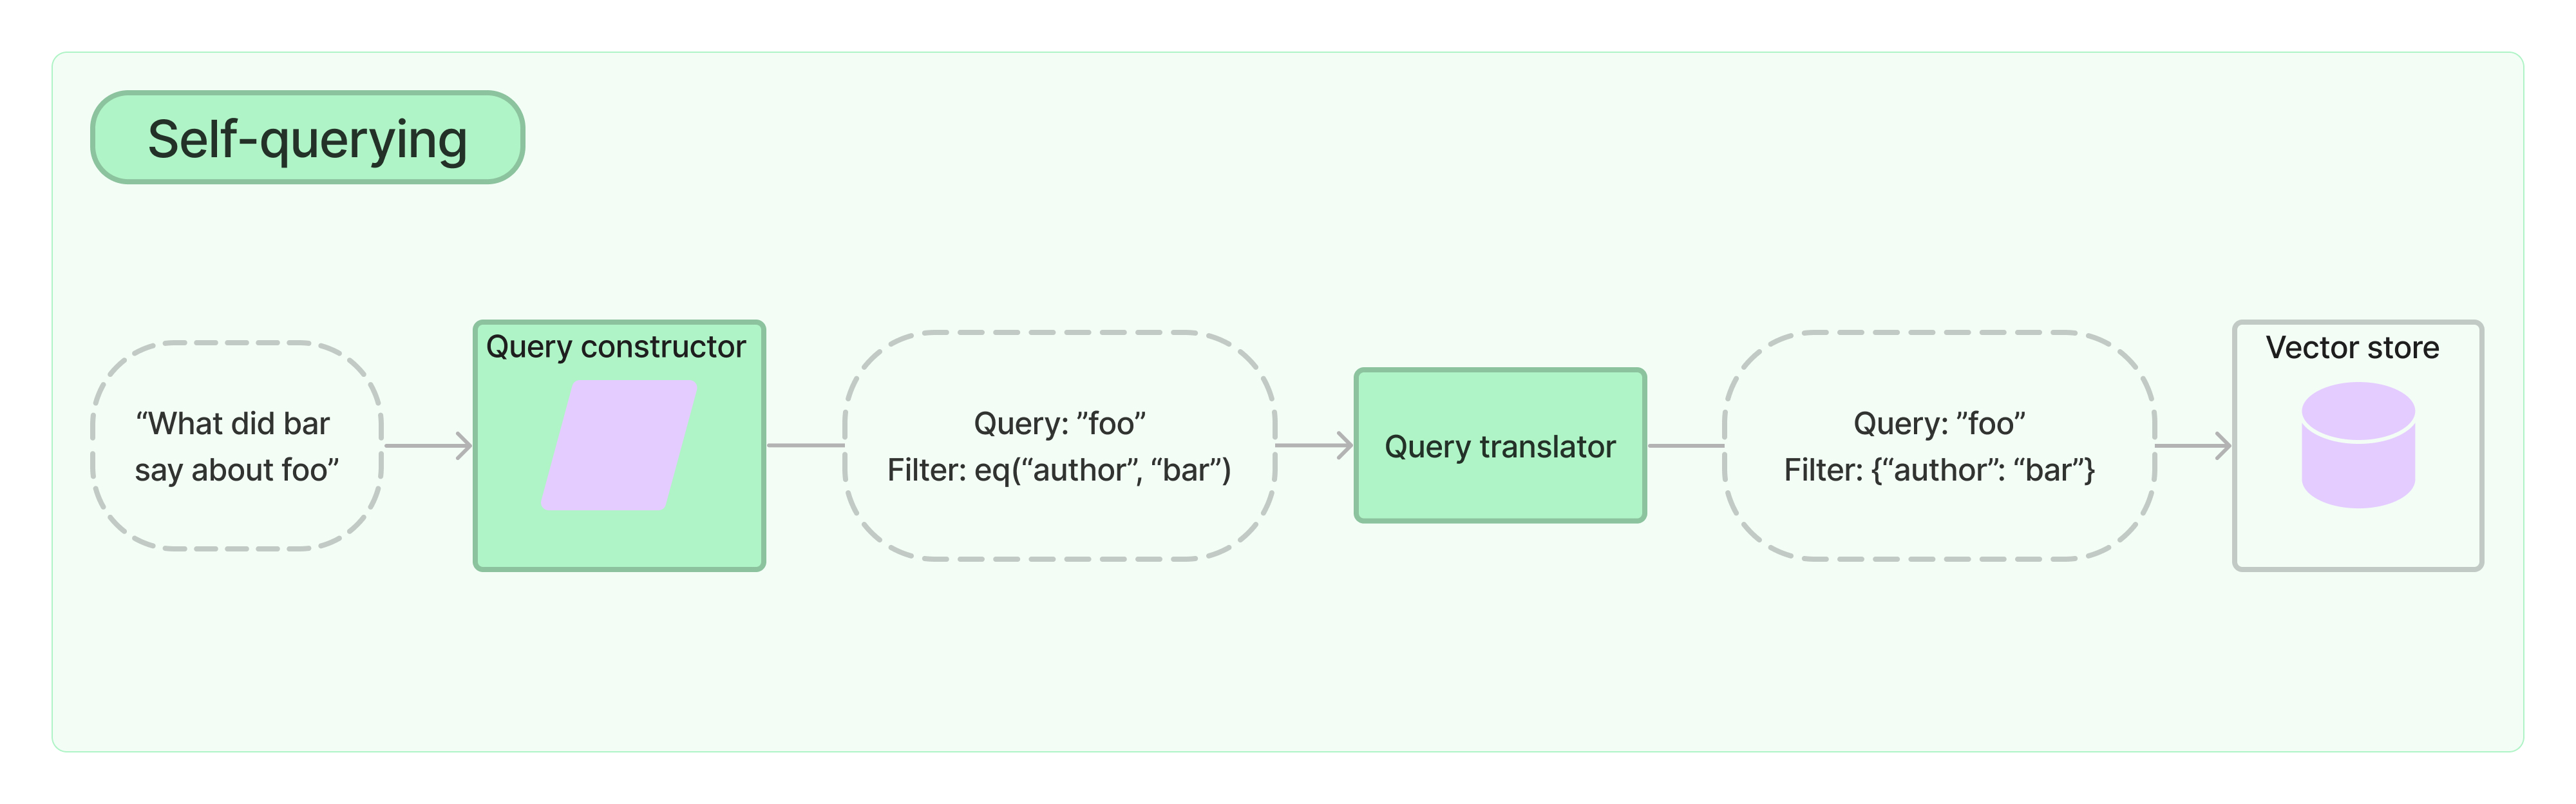
\includegraphics[width=0.7\pdfpagewidth]{images/selfquery.jpg}\label{fig:selfquery}
    \caption[Ingestion]{Come funziona un sistema di selfquerying.}
\end{figure}

Tali documenti vengono poi passati ad una catena di question answering, come contesto e, nella implementazione scelta, vengono presi in considerazione dal modello di OpenAI ``text-davinci-003'' che ciclicamente migliora la risposta precedente (figura \ref{fig:refine}).
In output vengono restituiti i documenti che il modello ha preso in considerazione e la risposta finale.

\begin{figure}
    \centering
    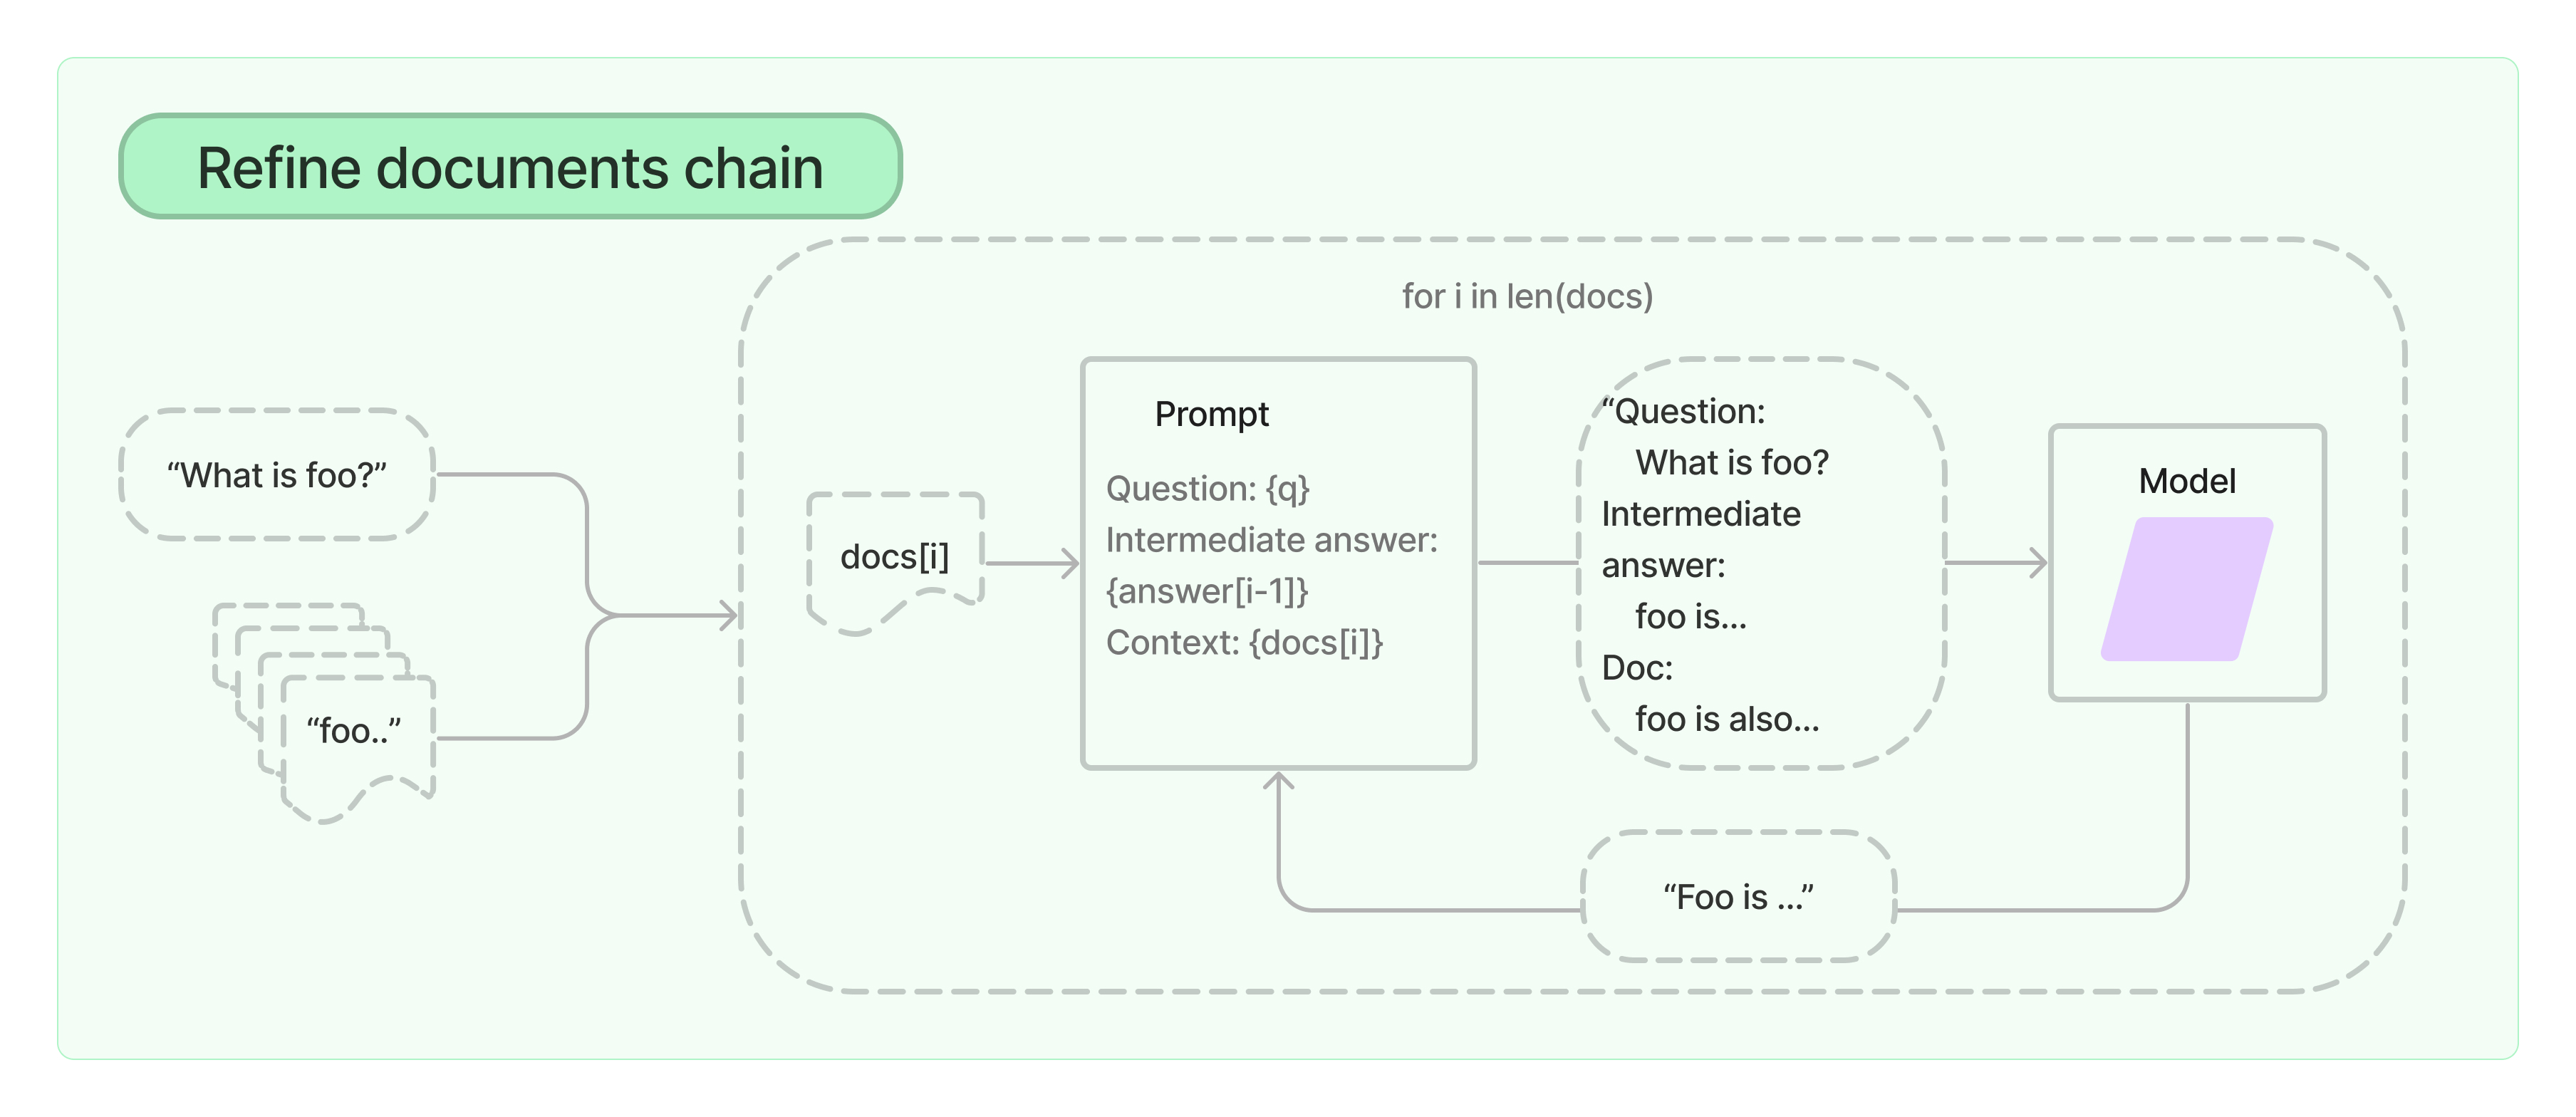
\includegraphics[width=0.7\pdfpagewidth]{images/refine.jpg}\label{fig:refine}
    \caption[Ingestion]{Come funziona una chain di tipo refine.}
\end{figure}


% \section{I risultati}
\subsection{Le query}
La costruzione delle query da sottoporre alla chain di question answering avviene tramite un json molto semplice che contiene solo la chiave "query" con dentro sotto forma di stringa la richiesta da effettuare.
\begin{lstlisting}[firstnumber=1]
    {
        "query": "Who won the battle of Hastings?"
    }
\end{lstlisting}

Tale modalità rende facile la comunicazione con un eventuale sistema di frontend che si occupi di raccogliere le richieste dell'utente e di inviarle al sistema di question answering tramite, per esempio, un API REST.

\subsection{Il ragionamento della chain}

La chain impiega circa quindici secondi, con le modalità descritte in precedenza, a rispondere alla query.
Tale tempo è dovuto alla scelta di utilizzare una macchina non propriamente potente, quella base di google colab, e anche dal tempo di risposta delle API di OpenAI.
Entrambi i tempi sono riducibili investendo su un hardware più potente e utilizzando un modello in loco.

Per far ciò la chain prende in considerazione i 4 chunk di documenti che tramite similarity research risultano più vicini alla query e li passa al modello di OpenAI, che ciclicamente migliora la risposta.

Utilizzando langchain in modalità verbosa si può apprezzare il ragionamento che porta alla risposta finale:

\begin{lstlisting}[breaklines]
    > Entering new RefineDocumentsChain chain...


> Entering new LLMChain chain...
Prompt after formatting:
Context information is below. 
------------
<PRIMO DOCUMENTO>
------------
Given the context information and not prior knowledge, answer the question: Who won the battle of Hastings? Use only context informations.

\end{lstlisting}

Questo è il primo passaggio dell'algoritmo di Refine e il primo documento viene inserito all'interno della input per intero, sono presenti inoltre alcune informazioni che LangChain inserisce per istruire il modello a non fare più di ciò che gli si sta chiedendo, questo è un problema comune sopratutto quando si modifica un parametro particolare degli LLM che viene definito "temperatura" ed indica quanto il modello debba utilizzare la sua parte creativa per dare la risposta.

\begin{lstlisting}[breaklines]
    > Entering new LLMChain chain...
Prompt after formatting:
The original question is as follows: Who won the battle of Hastings? Use only context informations.
We have provided an existing answer: 
Duke William won the battle of Hastings.
We have the opportunity to refine the existing answer (only if needed) with some more context below.
------------
<Nth DOCUMENTO>
------------
Given the new context, refine the original answer to better answer the question. If the context isn't useful, return the original answer.

> Finished chain.
\end{lstlisting}

Questo è invece come avviene il processo di refine, come descritto in precedenza viene eseguito per ogni documento recuperato dal database vettoriale.

Alla fine ciò che si ottiene è la risposta finale, che in questo caso è:

\textit{Duke William won the battle of Hastings on October 14th, 1066, defeating the English army led by King Harold Godwinson and his brother, Tostig, and Norwegian forces led by King Harold Hardrada. His victory ultimately led to his coronation as King of England two months later on Christmas Day.}

\subsection{I documenti presi in considerazione}
Per ogni query e risultato è possibile ottenere la lista dei chunk presi in considerazione dal sistema, per rispondere a questa domanda i chunk appartenevano a due libri diversi PPN1736870556.pdf, il cui titolo è ``Egland's story'' del 1918 e PPN1736868691.pdf, il cui titolo è ``Outlines of British history'' del 1885.
Oltre al semplice nome viene restituita anche la pagina del libro nella quale quel chunk era contenuto oltre a tutti i metadati inseriti in fase di ingestion.
\section{Costi}
I costi di un sistema di information retrieval basato su LLM possono essere divisi in due tipologie: fissi e di utilizzo.

I costi fissi sono quelli che non dipendono dal numero di query effettuate, ma solo dal numero di documenti indicizzati e dalla loro lunghezza.

Per il lavoro di tesi sono state utilizzate le API di OpenAI per semplicità di utilizzo e anche perché non richiedono capacità computazionali in loco.

Le api di OpenAI inoltre hanno un diverso costo rispetto al modello utilizzato. 

Il costo di indicizzazione utilizzando i modelli di OpenAI è di:

\begin{center}
    \begin{tabular}{|c|c|}
        \hline
        Model	& Usage \\
        \hline
        Ada v2	& \$0.0001\/1000 tokens \\
        \hline
    \end{tabular}
\end{center}

OpenAI stessa mette a disposizione altri modelli di embeddings ma ne sconsiglia l'utilizzo.

Il costo totale dell'indicizzazione è stato intorno ai 60\$.

Per quanto riguarda invece il costo di utilizzo, OpenAI mette a disposizione diversi modelli con diversi costi descritti nella tabella seguente:

\begin{center}
    \begin{tabular}{|c|c|c|c|}
        \hline
        Family & Model	& Input cost & Output cost \\
        \hline
        GPT-4 & 8k context	& \$0.03 / 1000 tokens &  	\$0.06 / 1000 tokens \\
        \hline
        & 32k context	& \$0.06 / 1000 tokens &  	\$0.12 / 1000 tokens \\
        \hline
        GPT-3.5 Turbo & 4k context	& \$0.0015 / 1000 tokens &  	\$0.002 / 1000 tokens \\
        \hline
        & 16k context	& \$0.003 / 1000 tokens &  	\$0.004 / 1000 tokens \\
        \hline

        GPT-3 & davinci	& \$0.0120 \/ 1000 tokens &  	\$0.0120  \/ 1000 tokens \\
        \hline
    \end{tabular}
\end{center}



Se si fosse utilizzato un modello di LLM proprietario o di terze parti in modo diretto sarebbe stato necessario un server con una GPU per poter effettuare le query in modo efficiente. In tal caso i costi si sarebbero ammortizzati sul lungo periodo.



\section{Le conclusioni}

Nel lavoro di tesi è stato dimostrato come grazie alle più recenti tecnologie del deep learning e del NLP sia possibile realizzare una proof of concept di un sistema di information retrieval.
Nella PoC sono state utilizzate le tecnologie allo stato dell'arte nel momento in cui è stata realizzata e la facilità di utilizzo di librerie come langchain e le api di OpenAI rendono lo sviluppo di tali sistemi enormemente più rapido rispetto alla realizzazione di un sistema di IR classico. 

I grandi enti di ricerca, le biblioteche e le aziende che hanno tanti documenti trarrebbero enorme vantaggio dall'utilizzo di tale tecnologie e sebbene l'opinione pubblica si sia entusiasmata in pochissimo tempo per sistemi come ChatGPT, bisogna comunque stare attenti ai possibli risvolti etici e sociali che tali tecnologie possono avere.